\documentclass[../distribution_theory_notes.tex]{subfiles}
\begin{document}
\section{Aula 08 - 16 de Setembro, 2024}
\subsection{Motivações}
\begin{itemize}
	\item Convolução;
	\item O Melhor Parágrafo do Édinho;
	\item Teorema de Fubini-Tonelli.
\end{itemize}
\subsection{Convoluções e Fubini-Tonelli.}
Em continuidade ao nosso estudo do espaço das funções teste, \(\mathcal{C}_{c}^{\infty}(\Omega )\), estudaremos agora um método de construir funções deste espaço a partir do único exemplo que demos, ou seja,
\[
	\varphi (x) = \left\{\begin{array}{ll}
		e^{-\frac{1}{1-|x|^{2}}}, & \quad |x|<1 \\
		0,                        & |x|\geq 1
	\end{array}\right.,
\]
utilizando a operação chamada \textit{convolução}.
\begin{tcolorbox}[
		skin=enhanced,
		title=Observação,
		fonttitle=\bfseries,
		colframe=black,
		colbacktitle=cyan!75!white,
		colback=cyan!15,
		colbacklower=black,
		coltitle=black,
		drop fuzzy shadow,
		%drop large lifted shadow
	]
	A análise de Fourier, ou análise harmônica, é um conjunto de técnicas que visam representar ``funções'' de uma determinada classe por meio de somas (série de Fourier) ou integrais (integral de Fouriar) de ``funções especiais'' dentro daquela classe. Essas técnicas giram em torno de duas operações fundamentais: a \textit{convolução} e a \textit{transformada de Fourier}.
\end{tcolorbox}

A fim de introduzir as ideias e uma intuição para elas, consideremos o seguinte exemplo simplificado: sejam \(f, p:[a, b]\rightarrow \mathbb{R}\) funções integráveis e, para cada n natural, dividimos \([a, b]\) em n partes iguais, obtendo a partição
\[
	P_{n}: a=x_{0}<x_1<\dotsc <x_{n}=b,
\]
onde \(x_{i}=a + i (b-a)/n,\; i = 0,1,2,\dotsc ,n,\) ou \(x_{i}=x_{i-1}+(b-a)/n\) a partir do índice 1. Com isso,
\[
	\Delta x_{i}=\frac{b-a}{n},\quad i=1,2,\dotsc ,n.
\]
Escolhendo arbitrariamente pontos  \(\xi_{i}, \zeta_{i}\) em \([x_{i-1}, x_{i}]\), a \textbf{média ponderada} dos n valores \(f(\xi_1), f(\xi_2),\dotsc , f(\xi_{n})\) com ``pesos'' \(p(\zeta_1), p(\zeta_2), \dotsc , p(\zeta_{n})\) é o número:
\[
	M_{n}(f; p) \coloneqq \frac{1}{\sum\limits_{i=1}^{n}p(\zeta_{i})}\sum\limits_{j=1}^{n}f(\xi_{j})p(\zeta_{j}).
\]
Vale mencionar que, a rigor, os pesos deveriam ser
\[
	\frac{p(\zeta_1)}{\sum\limits_{}^{}p(\zeta_{i})}, \dotsc , \frac{p(\zeta_{n})}{\sum\limits_{}^{}p(\zeta_{i})},
\]
pois a soma deles deve ser igual a 1.
\begin{figure}[H]
	\begin{center}
		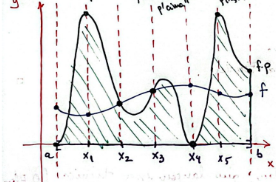
\includegraphics[height=0.5\textheight, width=0.5\textwidth, keepaspectratio]{./Images/weighted_avg_08.png}
	\end{center}
	\caption{os pesos ``puxam a média'' para cima.}
\end{figure}

Note que, multiplicando e dividindo \(M_{n}(f; p)\) por \((b-a)/n\), temos:
\[
	M_{n}(f; p)=\frac{1}{\sum\limits_{i=1}^{n}p(\zeta_{i})\frac{(b-a)}{n}}\sum\limits_{j=1}^{n}f(\xi_{j})p(\zeta_{j})\frac{(b-a)}{n} = \frac{1}{\sum\limits_{i=1}^{n}\Delta x_{i}}\sum\limits_{j=1}^{n}f(\xi_{j})p(\zeta_{j})\Delta x_{j},
\]
tal que, fazendo n tender a infinito e usando a continuidade de f e p, concluímos que
\[
	\lim_{n\to \infty}M_{n}(f; p)= \frac{1}{\int_{a}^{b}p(y) \mathrm{dy}}\int_{a}^{b}f(y)p(y) \mathrm{dy} \eqqcolon M(f; p).
\]
A média é um valor representativo de uma amostra, no sentido de representar alguma característica que se deseja analisar, então é razoável se definir a média ponderada dos valores de f com pesos p, também chamados \textbf{densidade}, em \([a, b]\) como esse limite. Em particular, se
\[
	\int_{a}^{b}p(y) \mathrm{dy}=1,
\]
então
\[
	M(f; p)=\int_{a}^{b}f(y)p(y) \mathrm{dy},
\]
sendo que, quando tanto f quanto p são não negativos, isto representa a área sob o gráfico de f. É claro que os maiores valores \(p(y)\) de p puxam a média para a média dos valores \(f(y)\) -- pode-se pensar que eles \textit{aumentam a influência}.

Para fixar estas ideias, consideramos o caso em que \([a, b]=[-1, 1]\), no qual p assume seu valor máximo em \(y=0\), p é não negativo no intervalo, \(\int_{-1}^{1}p \mathrm{dy} = 1\) e que seus valores sejam muito pequenos ``fora'' da origem; nestas condições, nosso objetivo é ver como isto ``puxa'' a média a fim de obtermos o valor \(f(0).\) Com efeito:
\begin{align*}
	M(f; p)-f(0) = \int_{-1}^{1}f(y)p(y) \mathrm{dy}-f(0) \cdot 1 & = \int_{-1}^{1}f(y)p(y) \mathrm{dy}-\int_{-1}^{1}f(0)p(y) \mathrm{dy}                                          \\
	                                                              & = \int_{-1}^{1}f(y)p(y)-f(0)p(y) \mathrm{dy}                                                                   \\
	                                                              & = \int_{-1}^{1}[f(y)-f(0)]p(y) \mathrm{dy}                                                                     \\
	                                                              & = \int_{-\delta }^{\delta }[f(y)-f(0)]p(y) \mathrm{dy} + \int_{|y|\geq \delta }^{}[f(y)-f(0)]p(y) \mathrm{dy}.
\end{align*}
Daí, vemos que, sendo f contínua em \(y_{0}=0,\; p\geq 0\) e \(\int_{}^{}p \mathrm{dy}=1\), a primeira parcela da igualdade acima tende a zero conforme \(\delta \) em si tende a zero; a segunda, como f é limitada e os valores de p são pequenos fora da origem, pode ser desprezada, o que sugere que nossa afirmação é correta: \(M(f; p)\) está próxima do valor \(f(0)\). Finalmente, se supormos que p é, além de tudo isso, uma função par com \(\mathrm{supp}(p)=[-1, 1]\) e que f esteja definida em toda a reta, podemos considerar os pesos ``móveis'' ponto a ponto, isto é, mover os pesos p ao longo da reta por meio das rotações \(r(y)=-y\) e translações
\[
	p_{x}(y)\coloneqq p(x-y) = p(y-x),
\]
sendo que
\[
	\mathrm{supp}(p_x)=[x-1, x+1],
\]
pois \(|x-y|\geq 1\) implica que \(p(x-y)=0\), tal que
\[
	p(x-y)\neq 0 \Rightarrow |y-x|\leq 1 \Rightarrow y\in [x-1, x+1].
\]
\begin{figure}[H]
	\begin{center}
		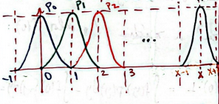
\includegraphics[height=0.5\textheight, width=0.5\textwidth, keepaspectratio]{./Images/density_08.png}
	\end{center}
	\caption{por meio de translações, os suportes de cada \(p_x\) são deslocados, mas mantêm a mesma forma.}
\end{figure}

Logo, a média
\[
	M(f; p_{x})= \int_{x-1}^{x+1}f(y)p_{x}(y) \mathrm{dy}=\int_{\mathbb{R}}^{}f(y)p(x-y) \mathrm{dy}
\]
é um valor aproximado do valor \(f(x).\) Observe que \(M(f; p_x)\) é uma função de x em \(\mathbb{R}\), no sentido de
\[
	x\mapsto M(f; p_x)
\]
e, se p for uma função \(\mathcal{C}^{\infty}\) com f apenas contínua (ou só integrável), o \textit{teorema da convergência dominada de Lebesgue} pode ser usado para provar que essa média é \(\mathcal{C}^{\infty}\) por meio da derivação sob o sinal de integração:
\[
	\frac{\mathrm{d}}{\mathrm{d}x} \int_{\mathbb{R}}^{}f(y)p(x-y) \mathrm{dy}=\int_{\mathbb{R}}^{}f(y) \frac{\mathrm{d}}{\mathrm{d}x}p(x-y) \mathrm{dy},
\]
ou seja, ela fornece um mecanismo para aproximar a função f por meio de funções \(\mathcal{C}^{\infty}\), nos fornecendo, assim, \textit{teoremas de densidade} em diversos espaços de funções integráveis. Os detalhes técnicos deste procedimento serão apresentados a seguir em algumas situações concretas, primeiro ``entre funções'' e segundo ``entre distribuições''.

Essas ideias também explicam que, ao calcular
\[
	p\mapsto \int_{}^{}f \varphi
\]
para uma função \(f\in L_{\mathrm{loc}}^{1}\) e \(\varphi \in \mathcal{C}_{c}^{\infty}\), estamos calculando uma média ponderada dos valores de f (multiplicada por \(\int_{}^{}\varphi \)) com peso \(\varphi \) ou, mais geralmente, se \(u\in \mathcal{D}',\) então
\[
	\varphi \mapsto \left< u, \varphi  \right>
\]
teria o mesmo significado, que é coerente com a física, a qual trabalha com médias dos valores obtidos de suas medições.

Para tudo o que se segue, a menos que explicitamente dito o contrário, a palavra ``mensurabilidade'' irá se referir à mensurabilidade Borel (conjuntos e funções) e dx indicará a medida de Lebesgue (no espaço euclidiano correspondente) definida na \(\sigma \)-álgebra de Borel. Além disso, a integral em \(\mathbb{R}^{n}\), ``\(\int_{\mathbb{R}^{n}}^{}\)'' será indicada por apenas \(\int\).
O caso mais geral, no qual consideramos a classe \(\mathcal{L}\) das funções Lebesgue mensuráveis e m a medida de Lebesgue nel definida, só se faz necessário quando precisarmos argumentar com medidas completas.
\begin{tcolorbox}[
		skin=enhanced,
		title=Observação,
		fonttitle=\bfseries,
		colframe=black,
		colbacktitle=cyan!75!white,
		colback=cyan!15,
		colbacklower=black,
		coltitle=black,
		drop fuzzy shadow,
		%drop large lifted shadow
	]
	Se f e g são Borel mensuráveis, então a função
	\begin{align*}
		F: & \mathbb{R}^{n}\times \mathbb{R}^{n}\rightarrow \mathbb{C} \\
		   & (x, y)\longmapsto F(x,y)=f(x-y)g(y)
	\end{align*}
	é mensurável, pois
	\[
		G(z, w)=f(z)g(w) = [M \circ (f, g)](z, w),\quad M(s, t)=st
	\]
	é contínua, \(S(x, y)=x-y\) é contínua e
	\begin{align*}
		j: & \mathbb{R}^{n}\times \mathbb{R}^{n}\rightarrow \mathbb{C}\times \mathbb{C} \\
		   & (z, w)\longmapsto j(z, w)= (f(z), g(w))
	\end{align*}
	é (\(\mathcal{B}_{\mathbb{R}^{n}}\times \mathcal{B}_{\mathbb{R}^{n}}, \mathcal{B}_{\mathbb{C}\times \mathbb{C}}\))-mensurável.
\end{tcolorbox}

\begin{def*}
	Sejam f, g funções mensuráveis em \(\mathbb{R}^{n}\) e a valores complexos. Para cada x em \(\mathbb{R}^{n}\), o \textbf{produto de convolução de f por g em x} é definido pela integral
	\[
		(f*g)(x)=(f*g)(x) = \int_{}^{}f(x-y)g(y) \mathrm{dy} = M(g; f_x)\int_{}^{}f(y) \mathrm{dy}. \quad \square
	\]
\end{def*}
Sempre que a mesma existir (\(p=\infty\) implica que \(f*g(x)\) existe para todo x em \(\mathbb{R}^{n}\)) e for um número. Nesse caso, pelo teorema de mudança de variáveis com difeomorfismos \(h(z)=x-z\), onde z está em \(\mathbb{R}^{n}\), resulta que
\[
	f*g(x)=\int_{}^{}f(x-y)g(y) \mathrm{dy} = \int_{}^{}f(z)g(x-z) \mathrm{dz},
\]
ou seja, * é uma multiplicação comutativa:
\[
	f*g(x)=g*f(x).
\]
\begin{tcolorbox}[
		skin=enhanced,
		title=Lembrete!,
		after title={\hfill Fubini-Tonelli},
		fonttitle=\bfseries,
		sharp corners=downhill,
		colframe=black,
		colbacktitle=yellow!75!white,
		colback=yellow!30,
		colbacklower=black,
		coltitle=black,
		%drop fuzzy shadow,
		drop large lifted shadow
	]
	\begin{theorem*}[Fubini-Tonelli]
		\hypertarget{fubini_tonelli}{Sejam}\((X, \mathcal{M}, \mu )\) e \((Y, \mathcal{N}, \nu)\) dois espaços de medidas \(\sigma \)-finitas e f uma função \( \mathcal{M} \otimes \mathcal{N}\)-mensurável (\(f:X\times Y\rightarrow \mathbb{C}\) mensurável no produto \(\mathcal{M}\otimes \mathcal{N}\) ou segundo ele). Então, temos:

		\textbf{\underline{Tonelli}:} se \(f\geq 0\), então as funções \(g(x)=\int_{}^{}f(x, y) \mathrm{d}\nu(y)\) e \(h(y)=\int_{}^{}f(x, y) \mathrm{d}\mu(x)\) são mensuráveis em \(\mathcal{M}\) e \(\mathcal{N}\) respectivamente, e vale
		\begin{align*}
			\int_{X\times Y}^{}f \mathrm{d}(\mu \times \nu ) = \int_{X}^{}\biggl[\int_{Y}^{}f(x, y) \mathrm{d}\nu (y)\biggr] \mathrm{d}\mu(x) & = \int_{X}^{}g(x) \mathrm{d}\mu (x)                                              \\
			                                                                                                                                  & = \int_{Y}^{}\biggl[\int_{X}^{}f(x, y) \mathrm{d}\mu (x)\biggr] \mathrm{d}\nu(y) \\
			                                                                                                                                  & = \int_{Y}^{}h(y) \mathrm{d}\nu (y).
		\end{align*}
		Equivalentemente, isto é o mesmo que dizer que \(f_x:Y\rightarrow \mathbb{C},\; f_x(y)=f(x, y)\) e \(f^{y}:X\rightarrow \mathbb{C},\; f(x, y)\) são \(L^{1}(\nu )\) e \(L^{1}(\mu )\), respectivamente.

		\textbf{\underline{Fubini}:} se \(f\in L^{1}(\mu \times \nu )\), então \(g(x)\) é finito \(\mu\)-q.t.p., \(h(y)\) é finito \(\nu\)-q.t.p. Além disso, \(g\in L^{1}(\mu ),\; h\in L^{1}(\nu )\) e a igualdade acima se verifica.
	\end{theorem*}
\end{tcolorbox}

\begin{tcolorbox}[
		skin=enhanced,
		title=Lembrete!,
		after title={\hfill Desigualdade de Hölder},
		fonttitle=\bfseries,
		sharp corners=downhill,
		colframe=black,
		colbacktitle=yellow!75!white,
		colback=yellow!30,
		colbacklower=black,
		coltitle=black,
		%drop fuzzy shadow,
		drop large lifted shadow
	]

	\begin{theorem*}[Desigualdade de Hölder]
		\hypertarget{holder_inequality}{Dado} \(1\leq p\leq \infty\), seja \(p'\) tal que
		\[
			\frac{1}{p}+\frac{1}{p'}=1.
		\]
		Se \(f\in L^{p}(\mu )\) e \(g\in L^{p}(\mu )\), então \(fg\in L^{1}(\mu )\) com
		\[
			\Vert f \cdot g \Vert_{1}\leq \Vert f \Vert_p \cdot \Vert g \Vert_{p'}.
		\]
	\end{theorem*}

\end{tcolorbox}

A seguir, destacaremos algumas condições que asseguram a existência de \(f*g\) e demonstraremos alguns resultados:
\hypertarget{young_inequality}{
	\begin{theorem*}[Uma das Desigualdades de Young]
		Se \(f\in L^{1}(\mathbb{R}^{n})\) e \(g\in L^{p}(\mathbb{R}^{n}),\; 1\leq p\leq \infty\), então \(f*g(x)\) existe para quase todo ponto x em \(\mathbb{R}^{n}\). Além disso, \(f*g\in L^{p}(\mathbb{R}^{n})\) com
		\[
			\Vert f*p \Vert_{p}\leq \Vert f \Vert_{1} \cdot \Vert g \Vert_{p}.
		\]
	\end{theorem*}
}

\begin{proof*}
	Separaremos em casos:

	\textbf{\underline{p = \(\infty\)}:} como \(y\mapsto f(x-y)\) é \(L^{1}(y)\) e \(y\mapsto g(y)\) é \(L^{\infty}(y)\), para cada vetor x em \(\mathbb{R}^{n},\) o mapa
	\[
		y\mapsto f(x-y)\cdot g(y)
	\]
	é \(L^{1}(y)\) pela \hyperlink{holder_inequality}{\textit{Desigualdade de Hölder}} e vale que, para todo \(x\in \mathbb{R}^{n}\),
	\begin{align*}
		|f*g(x)|\leq \int_{}^{}|f(x-y)g(y)| \mathrm{dy} & \leq \biggl(\int_{}^{}|f(x-y)| \mathrm{dy}\biggr) \Vert g \Vert_{\infty}               \\
		                                                & =\Vert f \Vert_1 \cdot \Vert g \Vert_{\infty}                                          \\
		                                                & \Rightarrow \Vert f*g \Vert_{\infty}\leq \Vert f \Vert_1 \cdot \Vert g \Vert_{\infty}.
	\end{align*}

	\textbf{\underline{p = 1}:} Neste caso, o mapa
	\[
		(x, y)\mapsto f(x-y)g(y),\quad (x, y)\in \mathbb{R}^{n}\times \mathbb{R}^{n}
	\]
	é mensurável; consequentemente,
	\[
		(x, y)\mapsto |f(x-y)g(y)| \geq 0.
	\]
	Do \hyperlink{fubini_tonelli}{\textit{Teorema de Tonelli}},
	\[
		\int_{}^{}\biggl[\int_{}^{}f(x-y)g(y) \mathrm{dy}\biggr] \mathrm{dx}=\int_{}^{}\biggl[\int_{}^{}|f(x-y)| \mathrm{dx} \biggr]|g(y)| \mathrm{dy}= \int_{}^{}\Vert f \Vert_1 |g(y)| \mathrm{dy} = \Vert f \Vert_1 \cdot \Vert g \Vert_1 <\infty,
	\]
	mostrando que \((x, y)\mapsto f(x-y)g(y)\) é \(L^{1}(\mathbb{R}^{n}\times \mathbb{R}^{n})\), donde, do \hyperlink{fubini_tonelli}{\textit{Teorema de Fubini}},
	\[
		f*g(x)=\int_{}^{}f(x-y)g(y) \mathrm{dy}
	\]
	é finito em quase todo ponto \(x\in \mathbb{R}^{n}.\) Logo,
	\begin{align*}
		|f*g(x)| = |\int_{}^{}f(x-y)g(y) \mathrm{dy}| & \leq \int_{}^{}|f(x-y)||g(y)| \mathrm{dy}                                     \\
		                                              & \Rightarrow \int_{}^{}|f*g(x)| \mathrm{dx}                                    \\
		                                              & \leq \int_{}^{}\biggl[\int_{}^{}|f(x-y)||g(y)| \mathrm{dy}\biggr] \mathrm{dx} \\
		                                              & = \Vert f \Vert_1 \cdot \Vert g \Vert_1
	\end{align*}
	pelo que foi provado acima.

	\textbf{\underline{\(1<p<\infty\)}:} este caso decorre do anterior junto à \hyperlink{holder_inequality}{\textit{Desigualdade de Hölder}} mediante a seguinte observação: escrevendo
	\[
		|f(x-y)| |g(y)| = |f(x-y)|^{\frac{1}{p'}}\bigl[|f(x-y)|^{\frac{1}{p}} |g(y)|\bigr],\quad x, y\in \mathbb{R}^{n},
	\]
	note que, por f ser \(L^{1}\), então o mapeamento
	\[
		y\mapsto |f(x-y)|^{\frac{1}{p'}}
	\]
	está em \(L^{p'}(y)\) e
	\[
		y\mapsto |f(x-y)|^{\frac{1}{p}}|g(y)|
	\]
	está em \(L^{p}(y)\), para todos os vetores x em \(\mathbb{R}^{n}\), porque elevando-o a p, obtemos
	\[
		y\mapsto |f(x-y)||g(y)|^{p},
	\]
	que se enquadra no caso \(p=1\) já provado acima, tendo em vista que as duas partes do produto são \(L^{1}\). Consequentemente, isto nos dá
	\[
		\int_{}^{}|f(x-y)||g(y)|^{p} \mathrm{dy} = (|f|*|g|^{p}) < \infty
	\]
	para quase todo ponto \(x\in \mathbb{R}^{n}\), com
	\begin{align*}
		\int_{}^{}\biggl[\int_{}^{}|f(x-y)||g(y)|^{p} \mathrm{dy}\biggr] \mathrm{dx} & = \int_{}^{}(|f|*|g|^{p})(x) \mathrm{dx}       \\
		                                                                             & \leq \Vert f \Vert_1 \cdot \Vert g^{p} \Vert_1 \\
		                                                                             & = \Vert f \Vert_1 \Vert g \Vert_{p}^{p}.
	\end{align*}

	Finalmente, pela \hyperlink{holder_inequality}{\textit{Desigualdade de Hölder}}, concluímos que, para quase todo ponto x em \(\mathbb{R}^{n}\),
	\[
		y\mapsto |f(x-y)||g(y)| = \underbrace{|f(x-y)|^{\frac{1}{p'}}}_{\mathclap{\in L^{p'}(y)}}\underbrace{[|f(x-y)|^{\frac{1}{p'}}|g(y)|]}_{\mathclap{\in L^{p}(y)}}
	\]
	está em \(L^{1}(y)\), ou seja, existe o número
	\[
		f*g(x) = \int_{}^{}f(x-y)g(y) \mathrm{dy}
	\]
	para quase todo ponto \(x\in \mathbb{R}^{n}\), provando a primeira parte da conclusão.

	Com respeito à segunda parte, escrevemos
	\begin{align*}
		|f*g(x)|^{p} \leq \biggl(\int_{}^{}|f(x-y)g(y)| \mathrm{dy}\biggr)^{p} & = \biggl(\int_{}^{}|f(x-y)|^{\frac{1}{p'}}[f(x-y)^{\frac{1}{p}}|g(y)|] \mathrm{dy}\biggr)^{p}                                                                    \\
		                                                                       & \leq \biggl[\biggl(\int_{}^{}|f(x-y)| \mathrm{dy}\biggr)^{\frac{1}{p'}}\biggl(\int_{}^{}|f(x-y)||g(y)|^{p} \mathrm{dy}\biggr)^{\frac{1}{p}}\biggr]^{p}           \\
		                                                                       & = \Vert f \Vert_{1}^{\frac{p}{p'}} \int_{}^{}|f(x-y)||g(y)|^{p} \mathrm{dy}                                                                                      \\
		                                                                       & \Rightarrow \int_{}^{}|f*g(x)|^{p} \mathrm{dx} \leq \Vert f \Vert_{1}^{\frac{p}{p'}}\int_{}^{}\biggl[\int_{}^{}|f(x-y)||g(y)|^{p} \mathrm{dy}\biggr] \mathrm{dx} \\
		                                                                       & \leq \Vert f \Vert_{1}^{\frac{p}{p'}}\Vert f \Vert_1 \Vert g \Vert_{p}^{p}                                                                                       \\
		                                                                       & \Rightarrow \Vert f*g \Vert_p \leq \Vert f \Vert_{1}^{\frac{1}{p'}}\Vert f \Vert_{1}^{\frac{1}{p}}\Vert g \Vert_p = \Vert f \Vert_1 \Vert g \Vert_p,
	\end{align*}
	como queríamos. \qedsymbol
\end{proof*}
\begin{crl*}
	Se \(\varphi \in \mathcal{C}_c(\mathbb{R}^{n})\) e \(f\in L_{\mathrm{loc}}^{p}(\mathbb{R}^{n})\), então \(\varphi *f(x)\) existe para quase todo ponto x em \(\mathbb{R}^{n}.\)
\end{crl*}
\begin{proof*}
	Com efeito, dado \(x\in \mathbb{R}^{n}\), f está em \(L^{p}(\underbrace{x-\mathrm{supp}(\varphi )}_{\mathclap{\text{compacto}}})\). Noutras palavras,
	\[
		f \chi_{(x-\mathrm{supp}(\varphi ))}\in L^{p}(\mathbb{R}^{n}).
	\]
	Como
	\[
		\int_{\mathbb{R}^{n}}^{}|\varphi(y)| \mathrm{dy} = \int_{\mathrm{supp}(\varphi )}^{}|\varphi(y)| \mathrm{dy}
	\]
	e \(\varphi \in L^{1}(\mathbb{R}^{n})\), segue, portanto, que
	\[
		\varphi * f(x) = \int_{\mathbb{R}^{n}}^{}\varphi (x-y)f(y) \mathrm{dy} = \int_{\mathrm{supp}(\varphi )}^{}\varphi(x-y)f(y) \mathrm{dy}
	\]
	é finito para quase todo \(x\in \mathbb{R}^{n}.\) \qedsymbol

\end{proof*}
\end{document}
